\documentclass[nohyper,justified]{tufte-handout}\usepackage{graphicx, color}
%% maxwidth is the original width if it is less than linewidth
%% otherwise use linewidth (to make sure the graphics do not exceed the margin)
\makeatletter
\def\maxwidth{ %
  \ifdim\Gin@nat@width>\linewidth
    \linewidth
  \else
    \Gin@nat@width
  \fi
}
\makeatother

\definecolor{fgcolor}{rgb}{0.2, 0.2, 0.2}
\newcommand{\hlnumber}[1]{\textcolor[rgb]{0,0,0}{#1}}%
\newcommand{\hlfunctioncall}[1]{\textcolor[rgb]{0.501960784313725,0,0.329411764705882}{\textbf{#1}}}%
\newcommand{\hlstring}[1]{\textcolor[rgb]{0.6,0.6,1}{#1}}%
\newcommand{\hlkeyword}[1]{\textcolor[rgb]{0,0,0}{\textbf{#1}}}%
\newcommand{\hlargument}[1]{\textcolor[rgb]{0.690196078431373,0.250980392156863,0.0196078431372549}{#1}}%
\newcommand{\hlcomment}[1]{\textcolor[rgb]{0.180392156862745,0.6,0.341176470588235}{#1}}%
\newcommand{\hlroxygencomment}[1]{\textcolor[rgb]{0.43921568627451,0.47843137254902,0.701960784313725}{#1}}%
\newcommand{\hlformalargs}[1]{\textcolor[rgb]{0.690196078431373,0.250980392156863,0.0196078431372549}{#1}}%
\newcommand{\hleqformalargs}[1]{\textcolor[rgb]{0.690196078431373,0.250980392156863,0.0196078431372549}{#1}}%
\newcommand{\hlassignement}[1]{\textcolor[rgb]{0,0,0}{\textbf{#1}}}%
\newcommand{\hlpackage}[1]{\textcolor[rgb]{0.588235294117647,0.709803921568627,0.145098039215686}{#1}}%
\newcommand{\hlslot}[1]{\textit{#1}}%
\newcommand{\hlsymbol}[1]{\textcolor[rgb]{0,0,0}{#1}}%
\newcommand{\hlprompt}[1]{\textcolor[rgb]{0.2,0.2,0.2}{#1}}%

\usepackage{framed}
\makeatletter
\newenvironment{kframe}{%
 \def\at@end@of@kframe{}%
 \ifinner\ifhmode%
  \def\at@end@of@kframe{\end{minipage}}%
  \begin{minipage}{\columnwidth}%
 \fi\fi%
 \def\FrameCommand##1{\hskip\@totalleftmargin \hskip-\fboxsep
 \colorbox{shadecolor}{##1}\hskip-\fboxsep
     % There is no \\@totalrightmargin, so:
     \hskip-\linewidth \hskip-\@totalleftmargin \hskip\columnwidth}%
 \MakeFramed {\advance\hsize-\width
   \@totalleftmargin\z@ \linewidth\hsize
   \@setminipage}}%
 {\par\unskip\endMakeFramed%
 \at@end@of@kframe}
\makeatother

\definecolor{shadecolor}{rgb}{.97, .97, .97}
\definecolor{messagecolor}{rgb}{0, 0, 0}
\definecolor{warningcolor}{rgb}{1, 0, 1}
\definecolor{errorcolor}{rgb}{1, 0, 0}
\newenvironment{knitrout}{}{} % an empty environment to be redefined in TeX

\usepackage{alltt}
%\documentclass{article}
%\usepackage[absolute,showboxes]{textpos}
\usepackage[absolute]{textpos}
\usepackage{sidecap}
%\usepackage{color}
%\usepackage[usenames,dvipsnames,svgnames,table]{xcolor}
\IfFileExists{upquote.sty}{\usepackage{upquote}}{}
\begin{document}








\begin{wide}
\section{\Huge CIT1 : EURUSD : test : Short}
{\Large Trades file: \verb+BT2 EURUSD 75 Sells_ 01012012 31122012 2x+ }

\hrulefill 
\end{wide}

\begin{textblock*}{105mm}(105mm,46mm)
\begin{figure}
\vspace{0pt}
\begin{knitrout}
\definecolor{shadecolor}{rgb}{0.969, 0.969, 0.969}\color{fgcolor}
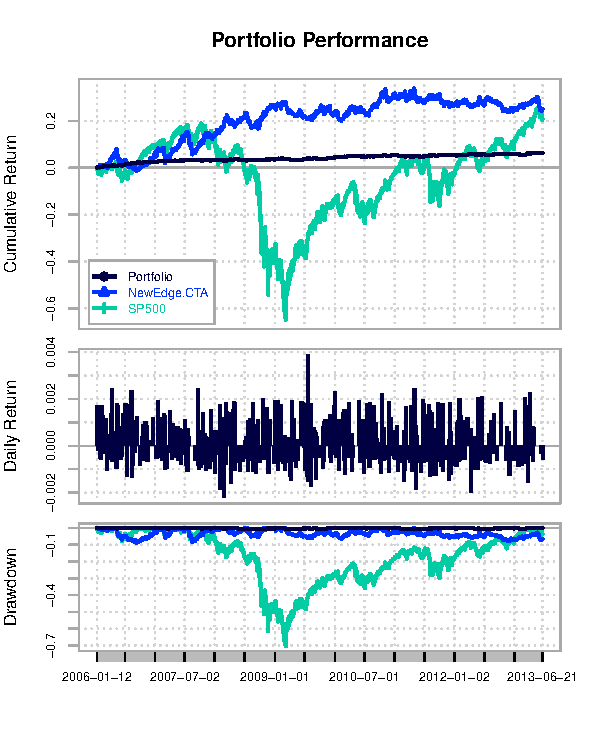
\includegraphics[width=\maxwidth]{figure/Performance} 

\end{knitrout}

\end{figure}
\end{textblock*}

\begin{textblock*}{95mm}(10mm,134mm)
\begin{figure}
\vspace{0pt}
\begin{knitrout}
\definecolor{shadecolor}{rgb}{0.969, 0.969, 0.969}\color{fgcolor}
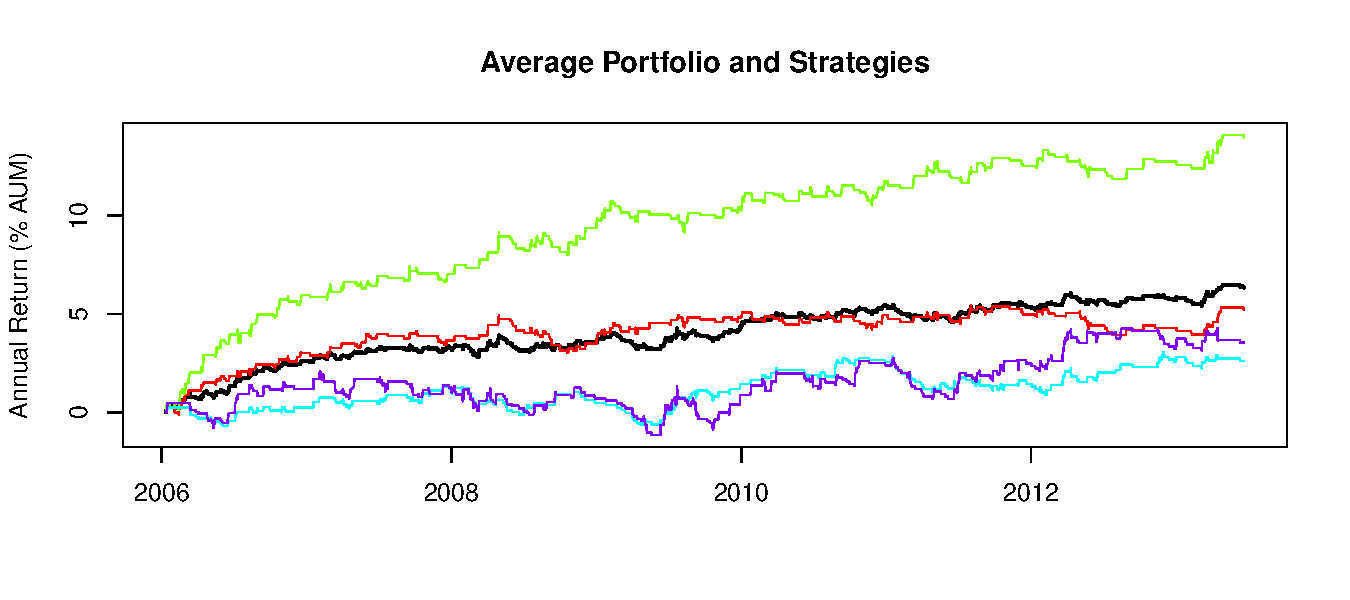
\includegraphics[width=\maxwidth]{figure/Performance2} 

\end{knitrout}

\end{figure}
\end{textblock*}


\begin{textblock*}{75mm}(15mm,55mm)
\Large Summary Statistics
\normalsize
%\newline
\begin{figure}
\vspace{0pt}


% latex table generated in R 2.15.2 by xtable 1.7-1 package
% Tue Jul 09 09:42:54 2013
\scalebox{0.7}{
\begin{tabular}{lr}
  \hline
 & Strategy \\ 
  \hline
Total Return (\% AUM) & -2.07 \\ 
  Compounded Annual Return (\%) & -2.12 \\ 
  Max Drawdown (\% AUM) & 2.06 \\ 
  Days to Recovery &  \\ 
  Max Consecutive Losing Trades & 12.00 \\ 
  Annualized Volatility (\%) & 1.51 \\ 
  Sharpe Ratio & -1.40 \\ 
  Sortino Ratio & -0.12 \\ 
  Kelly Fraction & -46.77 \\ 
  Total Return since 1 Jan 2010 (\% AUM) & -2.07 \\ 
  Total Return since 1 Jan 2011 (\% AUM) & -2.07 \\ 
  Total Return since 1 Jan 2012 (\% AUM) & -2.07 \\ 
   \hline
\end{tabular}
}


\end{figure}

\vspace{5mm}
\small Drawdown Length and Recovery Times
\normalsize
\begin{figure}
\begin{kframe}


{\ttfamily\noindent\bfseries\color{errorcolor}{\#\# Error: incorrect number of dimensions}}\end{kframe}

\end{figure}
\end{textblock*}


\begin{textblock*}{180mm}(15mm,170mm)
\begin{figure}
\vspace{0pt}
\begin{knitrout}
\definecolor{shadecolor}{rgb}{0.969, 0.969, 0.969}\color{fgcolor}
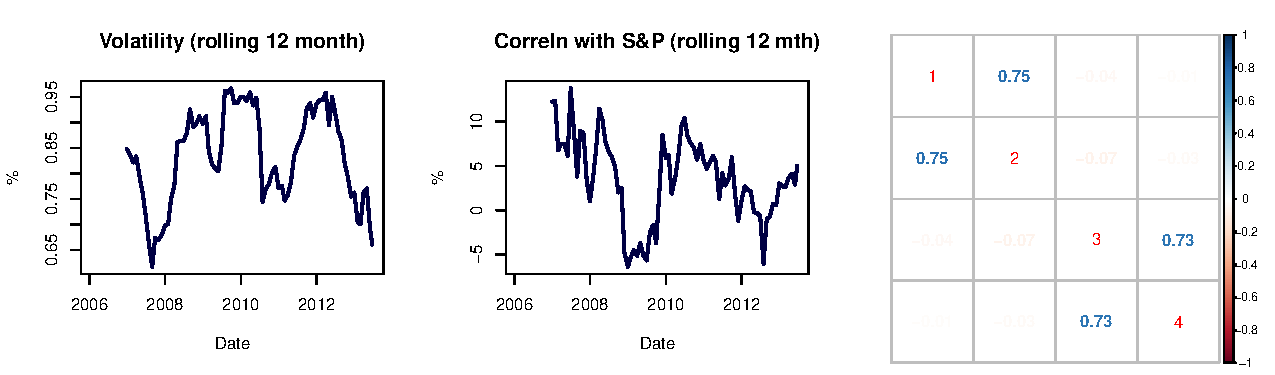
\includegraphics[width=\maxwidth]{figure/voletc} 

\end{knitrout}

\end{figure}
\end{textblock*}

\begin{textblock*}{180mm}(15mm,220mm)
\begin{figure}
\vspace{0pt}

\begin{knitrout}
\definecolor{shadecolor}{rgb}{0.969, 0.969, 0.969}\color{fgcolor}
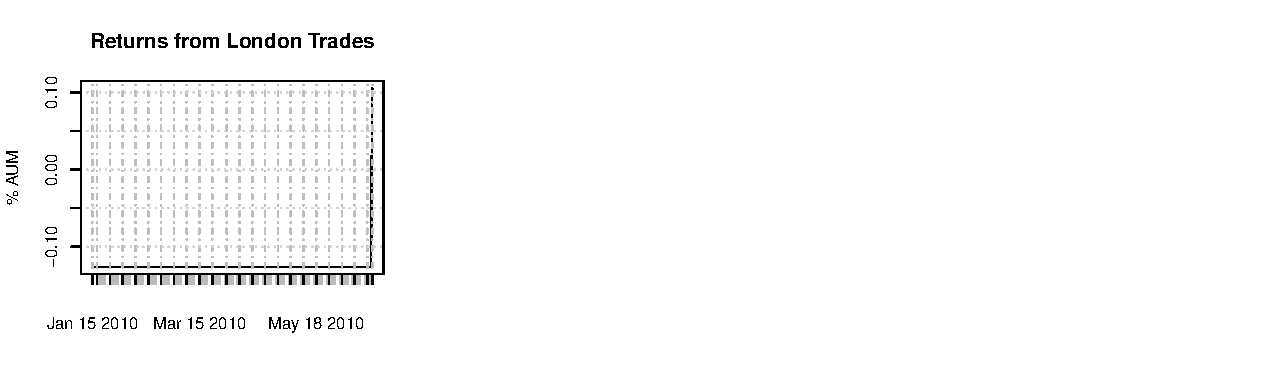
\includegraphics[width=\maxwidth]{figure/zonertns} 

\end{knitrout}

\end{figure}
\end{textblock*}



\end{document}
